\documentclass[conference]{IEEEtran}
\IEEEoverridecommandlockouts
\usepackage[utf8]{inputenc}
\usepackage[T1]{fontenc}
\usepackage{cite}
\usepackage{amsmath,amssymb,amsfonts}
\usepackage{algorithmic}
\usepackage{graphicx}
\usepackage{textcomp}
\usepackage{xcolor}
\def\BibTeX{{\rm B\kern-.05em{\sc i\kern-.025em b}\kern-.08em
    T\kern-.1667em\lower.7ex\hbox{E}\kern-.125emX}}
\begin{document}

\title{A Single Model for Enterprise and IoT Intrusion Detection: Cross-Domain Failure, Adversarial Robustness, and Edge Deployment}

\author{
\IEEEauthorblockN{\textit{Harishni A\textsuperscript{1*}, Kruthikha Vishali K\textsuperscript{1*}, Balasaraswathi V R\textsuperscript{1}}}
\IEEEauthorblockA{\textit{\textsuperscript{1}School of Computer Science and Engineering, VIT Chennai}\\
\textsuperscript{*}\textit{Both authors contributed equally to this work}}
}

\maketitle

\begin{abstract}
Enterprise and IoT network segments are conventionally secured by separate intrusion detection models. This approach fails badly under naive transfer: an enterprise-trained model applied zero-shot to IoT traffic scores AUC 0.264, worse than chance. A feature-ablation check traces a large part of this collapse to one feature whose relationship with the attack label reverses sign between domains --- a mechanism confirmed independently via SHAP and LIME and validated causally by retraining without it, though a smaller cross-domain gap remains unexplained. A single XGBoost model trained once on a canonical 15-feature schema pooling both domains nearly matches domain-specific performance (AUC 0.979/0.971) while improving IoT-side F1 (0.954 to 0.985), and outperforms two domain-adaptation baselines implemented head-to-head (CORAL; a DI-NIDS reimplementation), which reach only cross-domain AUC 0.35 to 0.69. Under a rigorous evaluation on n=548 confirmed pre-attack flows, a gradient-estimation attack (ZOO) evades only 18.4\%, but gradient-free and decision-based attacks evade 84 to 100\%, revealing a much larger evasion surface than a single attack family suggests. A SHAP-attribution drift monitor still flags the evaded traffic as a distributional shift (110x the alarm threshold). A cgroup-constrained Raspberry-Pi-4-class proxy shows the full pipeline (classify, explain, monitor) adds a bounded 4.1x latency increase (4.31 to 17.49 ms) within edge memory budgets. Results use bootstrap or Wilson 95\% confidence intervals, benchmarked against ten related studies, with limitations disclosed rather than a claim of unqualified success.
\end{abstract}

{\itshape Keywords --- Intrusion Detection, Domain Adaptation, XGBoost, SHAP, Adversarial Evasion, Population Stability Index, Edge Deployment}

\section{Introduction}

\subsection{Motivation and Problem Statement}

Today, modern networks suffer fundamentally different traffic regimes: an enterprise backbone and a fleet of IoT sensors experience different flow durations, header structures, and protocol mixes, even when both are compromised by the same broad attack families. The usual approach---training a separate, domain-specific intrusion detection model for each network segment---supposes that each model will generalise safely within its own domain and results in an operational overhead (since two models, two training pipelines, and two monitoring interfaces have to be maintained). This paper questions it directly, using two public, large-scale datasets that instantiate exactly this enterprise/IoT split: CSE-CIC-IDS2018 [1] (308,877 rows, enterprise) and CICIoT2023 [2] (297,091 rows sampled from a 46.7M-row source, IoT).

Cross-domain transfer of NIDS can fail catastrophically since the predictive relationship between a shared flow feature and the attack label may reverse when passing from one domain to another; however, when labeled data are available from both domains, an explicit domain-adaptation mechanism may not be necessary, since simple pooled training can avoid this kind of failure.

\subsection{Contributions}

Four primary contributions are made, each stated with an explicit number rather than a qualitative claim:

\begin{enumerate}

\item \textbf{A causally grounded account of naive cross-domain failure.} Applying an enterprise-trained model to IoT traffic zero-shot scores AUC 0.264 (below chance). Prior work (Layeghy \& Portmann [3]) has already traced comparable cross-domain collapses to SHAP-identified feature shifts; the contribution here is to independently confirm the specific inversion here with a second, unrelated method (LIME) and then test it causally: retraining without the implicated feature recovers a large part, but not all, of the lost AUC (Section V-B).

\item \textbf{A remedy that is simpler than what it out-performs.} A single XGBoost model trained once on a pooled, canonical 15-feature schema (AUC 0.979 / 0.971 on Enterprise / IoT respectively) outperforms both a CORAL domain-alignment baseline and a from-scratch reimplementation of DI-NIDS's [4] domain-adversarial-network + one-class-SVM architecture, evaluated on the same data for a genuine head-to-head rather than a cross-dataset citation.

\item \textbf{An uncertainty-quantified, three-attack-method adversarial evasion analysis at n = 548.} Results demonstrate that a gradient-estimation attack (ZOO, 18.4\% evasion) systematically underestimates the true vulnerability of tree-ensemble classifiers relative to gradient-free discrete random search, which exposes an 84--100\% evasion surface (Section V-D); this finding is corroborated with a second gradient-dependent attack (HopSkipJump), and shows that a SHAP-drift monitor still flags the resulting evaded traffic as a batch-level distributional shift by a wide margin.

\item \textbf{A reproducible, uncertainty-quantified edge-deployment benchmark}, reporting p50/p95/p99 latency percentiles under a real resource-constrained profile, benchmarked directly against three comparable studies.

\end{enumerate}

Headline results are reported with bootstrap or Wilson 95\% confidence intervals, or 5-seed mean $\pm$ standard deviation where applicable.

\section{Literature Survey}

\textbf{Cross-domain generalization.} The most similar work using these two datasets is Elangovan et al. [5], whose multi-dataset study reports a milder Macro-F1 degradation (0.69--0.78) under naive transfer than the AUC collapse found here (addressed directly in Section V-A). Cantone et al. [6] report substantial cross-dataset MCC/generalization collapse diagnosed via ad hoc data-visualization analysis, and Layeghy \& Portmann [3] independently report the same collapse pattern using SHAP-traced feature-shift explanations. Vitorino et al. [7] motivate percentile-bounded perturbation design for realistic network-intrusion adversarial examples, a principle behind the $\varepsilon$-budget bounding used here.

\textbf{SHAP-based explainability and drift.} Nugraha et al. [8] provide a clean template for SHAP-based NIDS explainability (F1 $\geq$ 99\% on three datasets). Tziouvaras et al. [9] establish PSI's provenance as a distributional-monitoring statistic in a wireless-network setting; to the authors' knowledge, no prior work applies PSI to SHAP-value vectors from a NIDS classifier and reuses one monitor unchanged across novel-attack-type and cross-domain-shift detection. Slack et al. [10] show SHAP and LIME explanations can themselves be adversarially manipulated by an attacker explicitly targeting the explanation method --- the drift-monitor result here holds against attackers targeting the classifier's decision, not the explanation itself. Wang et al. [11] similarly pair an ML-based IDS with an explainability layer. Barrett et al. [12] propose a conformal-prediction-based adaptive drift estimator for streaming intrusion detection, complementary to rather than overlapping with the batch-level SHAP-attribution monitor here.

\textbf{Adversarial robustness of tree ensembles.} Kantchelian et al. [13] established that tree ensembles have piecewise-constant, non-differentiable decision surfaces against which gradient-based attacks fail structurally. Rajhans \& Khawarey [14] demonstrate the same pathology for ZOO against XGBoost (Robustness Index 0.88--0.98 under ZOO vs. 0.30--0.44 under Square Attack [15] on the same models). Chen et al. [16] introduce HopSkipJump, a decision-based attack requiring only hard labels rather than gradients or confidence scores, evaluated here as a third attack family alongside ZOO and Square Attack.

\textbf{Domain adaptation methods.} CORAL [17], [18] and DANN [19] are the two adaptation mechanisms implemented and tested directly. Mahbub et al. [20] independently benchmark CORAL against a proposed alternative for cross-domain IoT/IoMT NIDS and likewise find CORAL underperforms, corroborating the negative CORAL result here (Section V-C). Wu et al. [21] report a heterogeneous open-set domain-adaptation approach for the network$\rightarrow$IoT direction specifically, targeting the same transfer direction studied here.

\textbf{Edge/lightweight deployment and data quality.} Almahaqeri et al. [22] and Ahmed et al. [23] both report near-ceiling XGBoost-family results on CICIoT2023 despite proposing new hybrid methods. Engelen et al. [24] report comparable data-quality issues in CICIDS2017, and Sarhan et al. [25] argue for the standard-feature-set methodology followed in Section III-A.

\section{Datasets}

\subsection{Dataset Description and Canonical Schema}

Enterprise coverage spans all 14 attack categories at a 44.2\% attack rate, versus all 34 IoT labels (33 attack + benign) at 96.6\%. The two datasets are extracted by different tools (CICFlowMeter true-flow features for CIC-IDS2018; fixed 10-or-100-packet traffic-aggregate windows, not true bidirectional flows, for CICIoT2023 --- verified against Neto et al.'s own methodology [2]) and cannot be modeled jointly without unification. Following the standard-feature-set methodology of Sarhan et al.~[25], a canonical 15-feature schema shared by both is defined --- duration, pkt\_len\_min/max/mean/std, total\_bytes, byte\_rate, header\_len\_total, five TCP flag indicators, is\_tcp, is\_udp --- with continuous fields log1p-transformed. Two features (header\_len\_total, byte\_rate) carry semantic, not just scale, mismatches between the two source extractors, retained because they still carry real predictive signal in both domains.

\subsection{Data-Integrity Checks}

Two duplicate/leakage checks were performed at two different levels of scope: a narrow check (exact-duplicate feature vectors between the IoT test and training partitions on the canonical schema) found 2.04\% cross-partition leakage, whether the training set was IoT-only or pooled Enterprise+IoT, which does not explain the performance difference between the two (Section V-A). Separately, Tolay [26] reports 54.82\% whole-corpus internal duplication across the full raw 46.7M-row CICIoT2023 release, a much broader question than the narrower test-vs-train check. Tolay's audit was independently recomputed from scratch on the full raw release by hashing all 39 raw feature columns per row, obtaining 54.99\% --- a near-exact replication.

The train/test split of CIC-IDS2018 also has a much higher rate of exact-duplicate-with-training on the Enterprise side (31.96\% of test rows have an identical twin in training, a documented dataset characteristic) than the 2.04\% IoT figure, so the headline models were re-evaluated after removing all exact-duplicate test rows: AUC shifted by at most 0.0015 and F1 by at most 0.0126 across all four model/domain combinations --- the headline results in Section V-A are qualitatively unchanged under de-duplicated evaluation.

\section{Proposed Work}

\subsection{System Overview}

Fig. 1 summarizes the overall pipeline. Enterprise and IoT traffic are first unified onto the canonical 15-feature schema (Section III-A), then used to train three XGBoost classifiers for a controlled head-to-head comparison. The resulting pooled model is then explained (SHAP + LIME), stress-tested against three adversarial attack families, monitored with a SHAP-attribution drift statistic, and benchmarked under a resource-constrained edge profile.

\begin{figure}[htbp]

\centerline{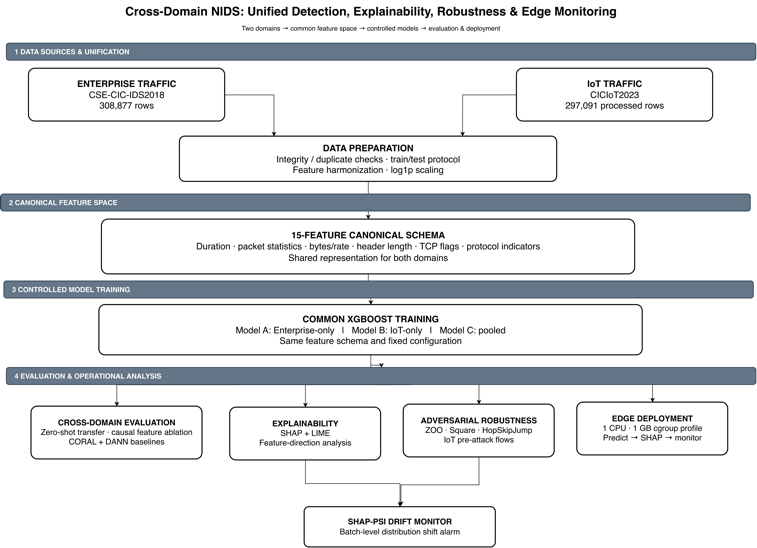
\includegraphics[width=0.48\textwidth]{fig1.png}}

\caption{Pipeline: two domains are unified on one canonical schema, three models are trained head-to-head, and the resulting classifier is explained, attacked, monitored, and benchmarked at the edge.}

\label{fig1}

\end{figure}

\subsection{Model Training: Three Models, One Schema}

Three XGBoost [27] classifiers are trained on the identical canonical schema: \textbf{Model A} (Enterprise-only), \textbf{Model B} (IoT-only), and \textbf{Model C} (pooled Enterprise+IoT, one training run), the proposed remedy. All three share the same manually-set hyperparameters (max depth 4, 200 estimators, histogram tree method, binary-logistic objective) with a class-imbalance-corrected \textit{scale\_pos\_weight}; no randomized or grid hyperparameter search was performed, so the reported numbers should be read as a fixed-configuration comparison rather than each model's fully-tuned ceiling. All headline metrics are reported with bootstrap 95\% confidence intervals (2,000 resamples of the fixed test set, percentile method).

\subsection{Domain-Adaptation Baselines}

To test whether a more sophisticated method is needed instead of simple pooling, two domain-adaptation baselines are implemented from scratch rather than only citing published numbers. \textbf{CORAL} [17], [18]: the 8 continuous canonical features are whitened per-domain using each domain's own training covariance, then recolored to a shared pooled covariance, before training the same XGBoost architecture on the aligned combined data. \textbf{DI-NIDS reimplementation (DANN + One-Class SVM)} [4]: a domain-adversarial neural network (gradient-reversal feature extractor, source-only label classifier, both-domains domain classifier, feature extractor 15$\rightarrow$32$\rightarrow$16 with sigmoid nonlinearity matching their formulation, progressive gradient-reversal schedule [19]) followed by a one-class SVM [28] on the resulting embeddings, trained under their actual unsupervised protocol in which target-domain labels are never used --- a strictly harder problem than Model C's pooled-label setting. Five seeds are run per transfer direction. This comparison is reported not to claim algorithmic superiority over a method solving a harder problem, but to answer a narrower, practically relevant question: when an organization already has labeled data in both domains (the setting here), does a more sophisticated domain-adaptation mechanism still earn its complexity over simple pooled training? Section V-C shows it does not.

\subsection{Explainability Protocol}

SHAP [29] attributions are computed for Model C in both domains using TreeExplainer, the model-specific algorithm underlying SHAP's tree-ensemble speedup [30], over 500 test instances per domain. To cross-validate any mechanistic claim derived from SHAP against a second, mechanistically unrelated method, the analysis is repeated with LIME [31], a perturbation-sampled local-surrogate method, using the same 500 instances per domain and 5,000 perturbation samples per explained instance.

\subsection{Adversarial Robustness Evaluation}

Three black-box attack families are evaluated on a fixed subset of 548 confirmed pre-attack IoT flows, a sample size chosen to keep evasion-rate confidence intervals narrow, using the Adversarial Robustness Toolbox [32]: \textbf{ZOO} [33], a gradient-estimation attack; a \textbf{Square-style} discrete random search implemented in-house for tabular data (ART's built-in Square Attack implementation is hard-coded for image tensors), with perturbations bounded relative to the original clean point at budgets $\varepsilon$ = 0.10 and $\varepsilon$ = 0.30 (L$\infty$, i.e.~the maximum absolute per-feature change is capped at that fraction of each feature's clipped range); and \textbf{HopSkipJump} (HSJ) [16], a decision-based attack that searches for the minimum L$\infty$ perturbation crossing the decision boundary via boundary-projection binary search plus Monte-Carlo gradient-direction estimation. All three are run under identical conditions to permit direct comparison. All perturbations are bounded per-feature only; cross-feature physical consistency is not enforced (e.g.~\textit{pkt\_len\_min} $\leq$ \textit{pkt\_len\_max}, or \textit{total\_bytes} scaling with \textit{byte\_rate}), so some adversarial examples may not correspond to packets a real network stack could emit --- a limitation disclosed explicitly rather than claiming the attacks are traffic-realistic.

\subsection{SHAP-Attribution Drift Monitor}

A Population Stability Index (PSI) monitor is built over Model C's SHAP-value vectors. For each of the 15 features, reference-distribution bin edges are the 10 deciles of that feature's SHAP values in a fixed reference batch; the same edges bin the comparison batch; the standard per-feature PSI, $\Sigma$(batch\_pct $-$ ref\_pct)$\cdot$ln(batch\_pct/ref\_pct), is computed on signed SHAP values directly; and the final scalar is the unweighted mean of the 15 per-feature PSI values. The alarm threshold is fixed before evaluating any shift condition, from 20 independent same-domain null draws only (threshold = 0.0125). The calibrated monitor is then tested against three qualitatively different distribution shifts: within-domain novel-attack-type generalization, Enterprise$\rightarrow$IoT domain shift, and the adversarially-evaded traffic from Section IV-E.

\subsection{Edge Deployment Benchmark}

The full three-tier pipeline (classify $\rightarrow$ +SHAP $\rightarrow$ +drift monitor) is benchmarked under a cgroup-constrained profile (1 CPU-core CFS quota, 1 GB memory cap) approximating a Raspberry-Pi-4-class device, following Diab et al.~[34] and Wijethilaka et al.~[35] in using constrained rather than unconstrained hardware. Mean, p50, p95, and p99 latency per tier, plus peak memory, are reported and compared directly against three other studies.

\section{Results and Discussion}

\subsection{Cross-Domain Performance}

\begin{table}[htbp]
\caption{Cross-domain AUC/F1, with 95\% bootstrap CI}
\begin{center}
\footnotesize
\resizebox{\columnwidth}{!}{%
\begin{tabular}{|c|c|c|}
\hline
\textbf{Model / condition} & \textbf{AUC (95\% CI)} & \textbf{F1 (95\% CI)} \\
\hline
A, in-domain (Enterprise) & 0.9816 [0.9807, 0.9825] & 0.9344 [0.9322, 0.9365] \\
\hline
B, in-domain (IoT) & 0.9738 [0.9717, 0.9758] & 0.9541 [0.9528, 0.9553] \\
\hline
A$\rightarrow$IoT, naive zero-shot & 0.2643 [0.2571, 0.2717] & 0.5487 [0.5447, 0.5527] \\
\hline
B$\rightarrow$Enterprise, naive zero-shot & 0.5525 [0.5479, 0.5570] & 0.6126 [0.6089, 0.6162] \\
\hline
\textbf{C, Enterprise test} & \textbf{0.9794 [0.9783, 0.9804]} & \textbf{0.9286 [0.9263, 0.9310]} \\
\hline
\textbf{C, IoT test} & \textbf{0.9709 [0.9684, 0.9731]} & \textbf{0.9849 [0.9842, 0.9856]} \\
\hline
\end{tabular}
}
\label{tab1}
\end{center}
\end{table}

Given large test sets (59k--72k rows), all intervals are tight; A$\rightarrow$IoT's 95\% CI of [0.257, 0.272] is nowhere close the chance level of 0.5, confirming the zero-shot collapse is a statistically robust finding. Model C incurs only a small Enterprise-side reduction relative to Model A (a paired bootstrap on the AUC difference gives $\Delta$AUC = 0.0023, 95\% CI [0.0019, 0.0027] --- real but small) while improving on Model B on IoT (F1 0.985 vs. 0.954 is a real gain), attributed to Enterprise data acting as regularization for IoT detection (Section V-B).

Because Elangovan et al.'s [5] Macro-F1 range (0.69--0.78) looks considerably gentler than the AUC collapse here, Macro-F1 was recomputed for the zero-shot models: A$\rightarrow$IoT Macro-F1 = 0.285, B$\rightarrow$Enterprise Macro-F1 = 0.306, both comparably severe to the AUC collapse and not rescued by a gentler metric. The discrepancy with Elangovan et al. is attributed to AUC --- being rank-based and threshold-free --- being more sensitive to the sign-inverted decision-rule mechanism identified in Section V-B than Macro-F1 is to preserved majority-class recall under domain shift.

\subsection{Explainability Results}

Spearman rank correlation of mean-|SHAP| feature importance between Enterprise and IoT domains for Model C is $\rho$ = 0.900 (p < 0.0001): the same handful of features (\textit{duration}, \textit{header\_len\_total}, \textit{pkt\_len\_max/min}, \textit{flag\_ack}) matter for detection in both domains (Fig. 2). This is not the same as a shared explanation vocabulary in the strong sense: \textit{duration} and \textit{header\_len\_total} alone predict \textit{domain} (Enterprise vs.~IoT) with AUC = 1.0000, and \textit{header\_len\_total}'s raw correlation with the attack label flips sign between domains (+0.061 Enterprise, $-$0.235 IoT). This provides a mechanistically supported explanation for the A$\rightarrow$IoT collapse: a decision rule learned in one domain (``long header $\rightarrow$ suspicious'') becomes misleading in the other.

To test this mechanism causally rather than only correlationally, Models A and B were retrained on the remaining 13 features only --- dropping \textit{header\_len\_total} and \textit{byte\_rate}, the two features Section III-A discloses as carrying semantic, not just scale, mismatches between the two extractors --- using identical hyperparameters (Section IV-B). Zero-shot AUC improves substantially without them (A$\rightarrow$IoT: 0.264 $\rightarrow$ 0.645; B$\rightarrow$Enterprise: 0.553 $\rightarrow$ 0.621) while in-domain performance is nearly unchanged (A: 0.982 $\rightarrow$ 0.978; B: 0.974 $\rightarrow$ 0.954), confirming these two features are large contributors to the collapse and providing causal support for the sign-flip mechanism above, beyond the earlier correlational evidence. A real cross-domain gap persists even after removing them (0.645/0.621 zero-shot vs.~$\approx$0.97 in-domain), indicating the two flagged features explain a large part, but not all, of the naive-transfer failure.

\begin{figure}[htbp]

\centerline{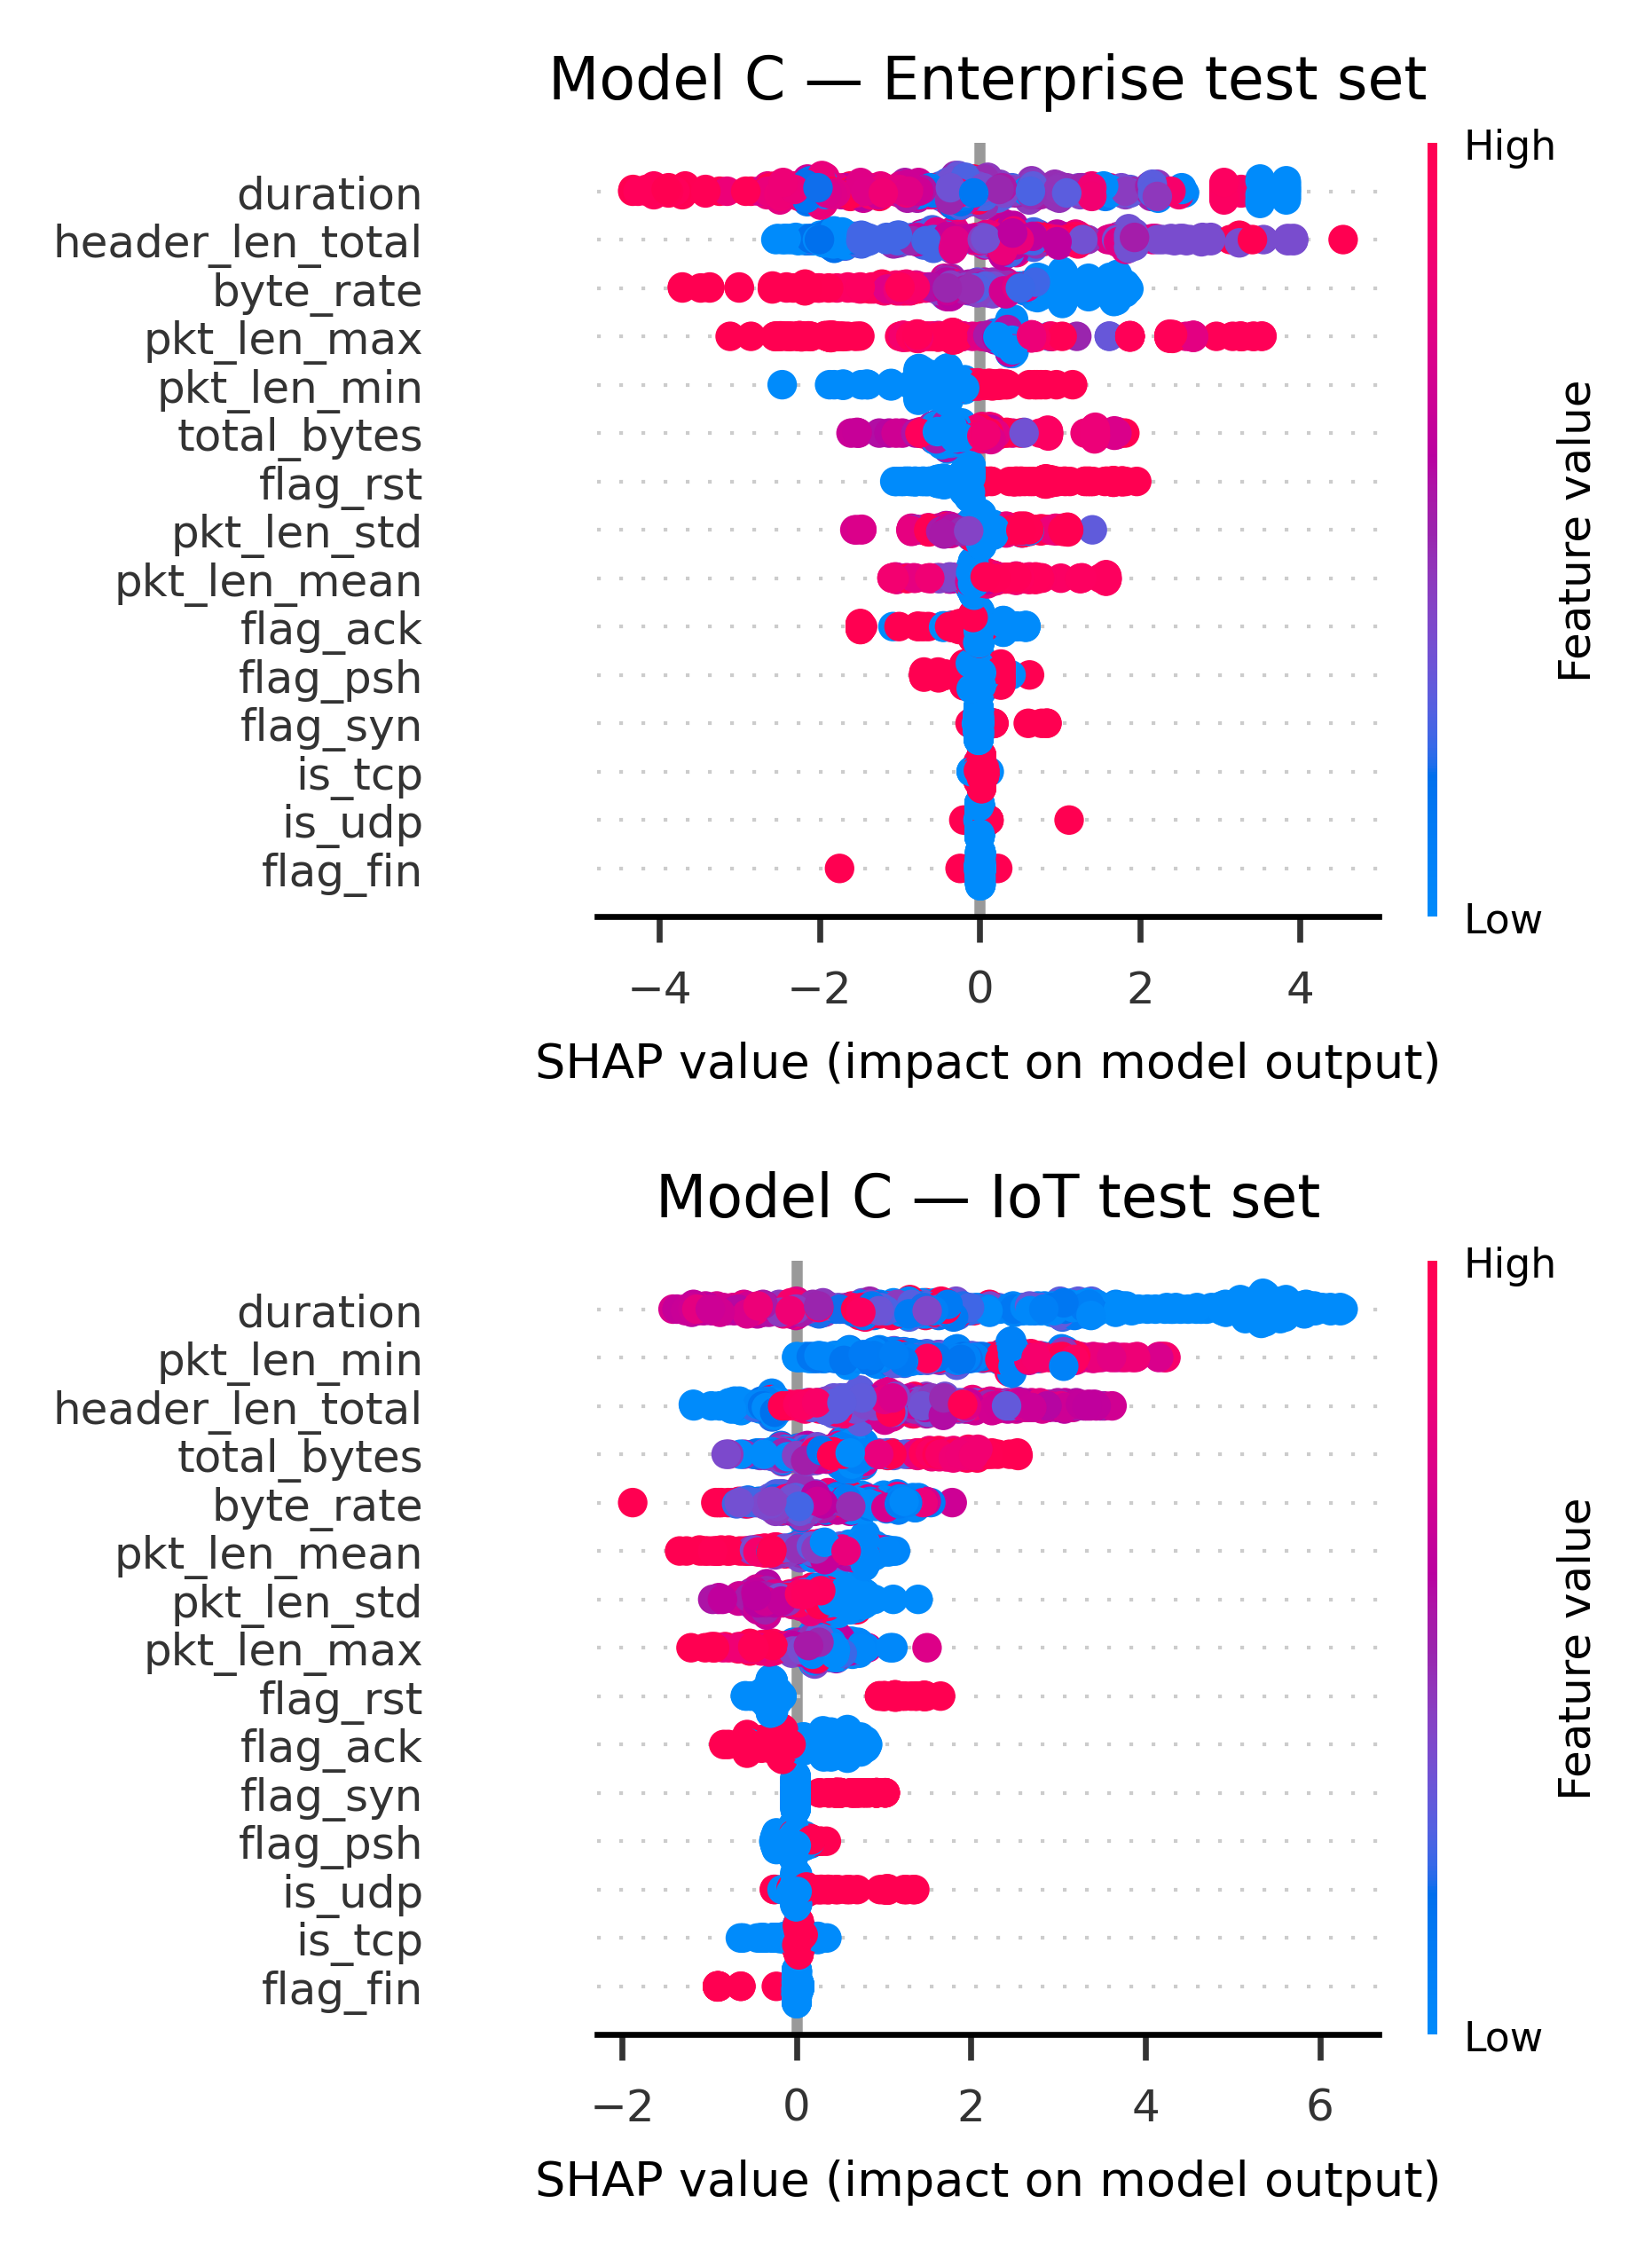
\includegraphics[width=0.48\textwidth]{fig2.png}}

\caption{SHAP summary plots, Model C, 500 test instances per domain.}

\label{fig2}

\end{figure}

\begin{table}[htbp]
\caption{SHAP vs.~LIME cross-validation of the sign-flip finding}
\begin{center}
\footnotesize
\begin{tabular}{|c|c|c|}
\hline
\textbf{Domain (model)} & \textbf{SHAP corr.} & \textbf{LIME corr.} \\
\hline
Enterprise (A) & +0.508 & +0.591 \\
\hline
IoT (B) & $-$0.916 & $-$0.511 \\
\hline
\end{tabular}
\label{tab2}
\end{center}
\end{table}

Both methods independently agree the direction flips for the domain-specific models --- the models that are actually naively transferred (Table II). A pooled Model C shows no such flip by either method.

\subsection{Domain-Adaptation Baseline Results}

On Enterprise, CORAL (AUC/F1 = .979/.928) $-$ Model C = +0.0001 AUC, 95\% CI [$-$0.0004, +0.0005] (a genuine tie), and on IoT, CORAL (.967/.983) $-$ Model C = $-$0.0039 AUC, 95\% CI [$-$0.0053, $-$0.0024] (small but real degradation) are obtained from a paired bootstrap (2,000 resamples, same test rows scored by both models). Explicit domain-invariance training via CORAL therefore does not improve on naive joint training, and on IoT specifically makes things measurably worse --- a less severe failure than Pawlicki et al.'s [36] independent CORAL result (target-domain F1 collapsing to 0.04).

\begin{table}[htbp]
\caption{DANN+OSVM reimplementation, 5-seed mean $\pm$ std}
\begin{center}
\footnotesize
\begin{tabular}{|c|c|c|c|c|}
\hline
\textbf{Direction} & \textbf{Src F1} & \textbf{Src AUC} & \textbf{CD F1} & \textbf{CD AUC} \\
\hline
Ent$\rightarrow$IoT & .81$\pm$.05 & .88$\pm$.03 & .77$\pm$.10 & .35$\pm$.13 \\
\hline
IoT$\rightarrow$Ent & .84$\pm$.02 & .86$\pm$.02 & .61$\pm$.00 & .69$\pm$.04 \\
\hline
\end{tabular}
\label{tab4}
\end{center}
\end{table}

\textit{(Src. = OSVM performance on the source domain's own held-out test set, i.e. the in-domain ceiling this method transfers from --- not a domain-discrimination check; CD = cross-domain transfer performance on the unlabeled target domain; Ent = Enterprise; values rounded to 2 d.p.)}

A sanity check confirms the adversarial training converged rather than collapsed: the domain classifier's held-out source-vs-target accuracy is 0.52 $\pm$ 0.03 / 0.51 $\pm$ 0.04, near the 50\% chance level a genuinely domain-invariant embedding should produce. Pooled training (Model C) prevails by a wide margin regardless (cross-domain AUC 0.97--0.98 vs. 0.35--0.69). DI-NIDS solves a strictly harder problem (zero target labels).

\subsection{Adversarial Evasion Results}

To reduce uncertainty associated with small sample sizes, the full evasion benchmark is assessed on 548 confirmed pre-attack IoT flows (\textit{is\_attack==1} test rows, fixed \textit{random\_state=42}, drawn from the same test set used throughout) using identical model, attack hyperparameters, and budgets across all three methods; ZOO evades 18.4\% (101/548), 95\% Wilson CI [15.4\%, 21.9\%].

\begin{figure}[htbp]

\centerline{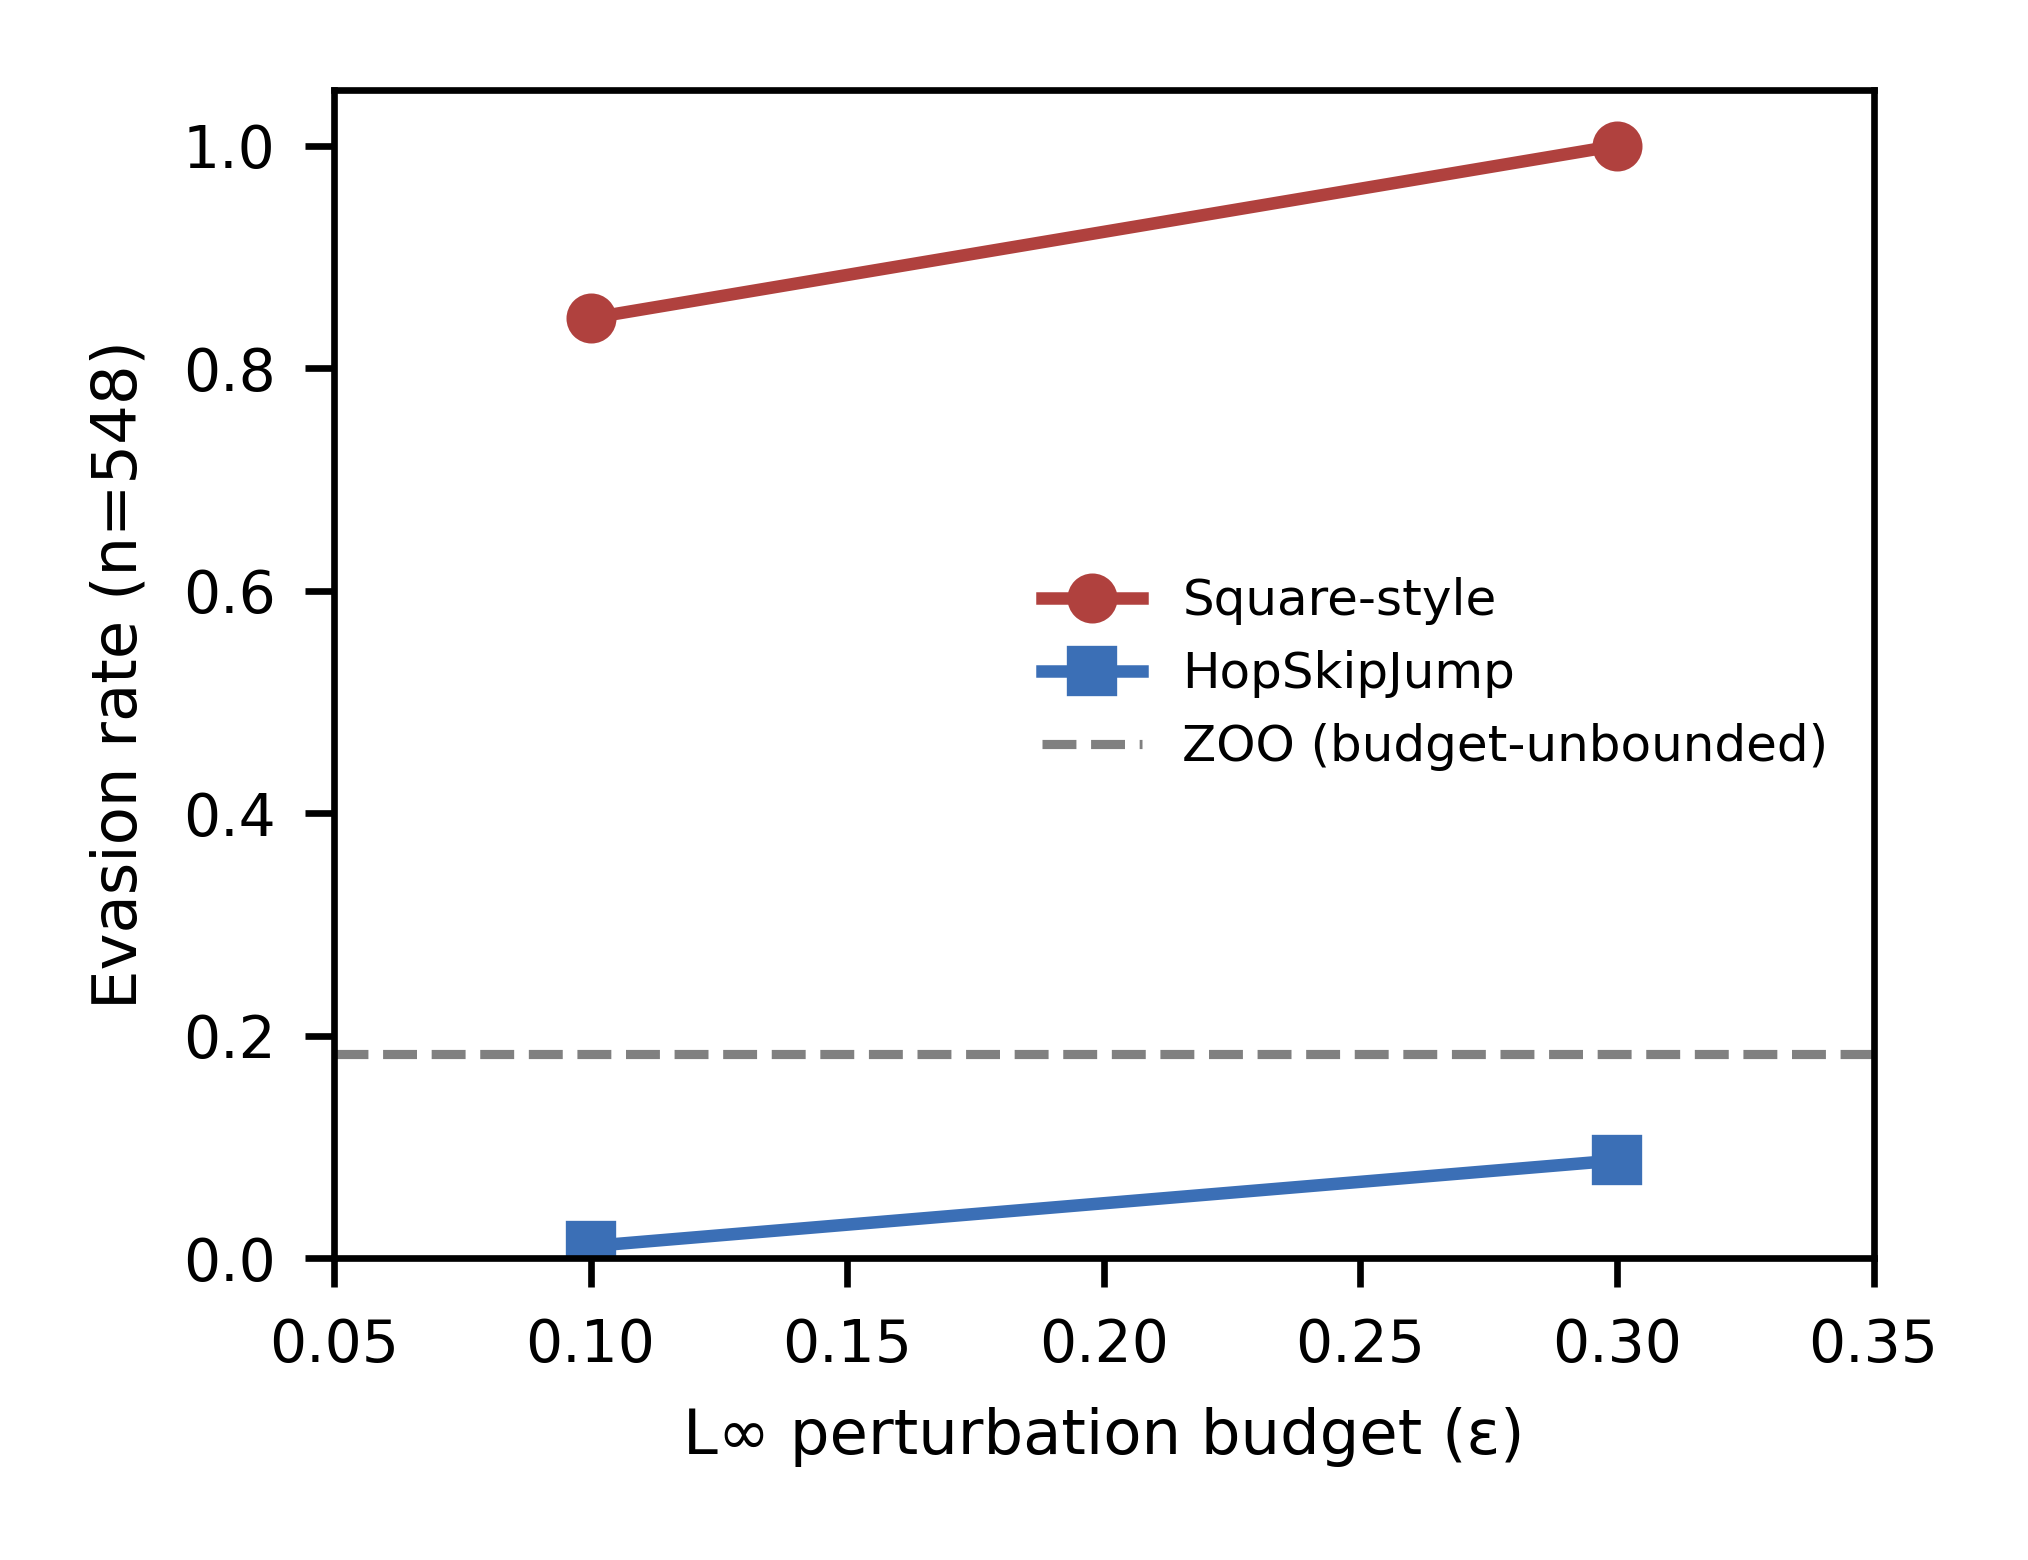
\includegraphics[width=0.48\textwidth]{fig3.png}}

\caption{Evasion rate vs.~perturbation budget, three attack families (n = 548).}

\label{fig3}

\end{figure}

Consistent with Rajhans and Khawarey's [14] discovery that gradient-estimation attacks systematically underestimate true vulnerability against tree ensembles, all 101 flows evaded by ZOO are also evaded by the Square-style attack at the larger budget ($\varepsilon$ $\leq$ 0.30, a strict subset). HopSkipJump's refinement step relies on the same class of numerically-estimated local direction information as ZOO against the same non-smooth decision surface; HopSkipJump only finds a small-perturbation route for 1.1\% [0.5, 2.4] of flows at $\varepsilon$ $\leq$ 0.10 and 8.8\% [6.7, 11.4] at $\varepsilon$ $\leq$ 0.30, the same small budgets where Square-style already achieves 84.5\% [81.2, 87.3] and 100\% [99.3, 100] evasion respectively, but it eventually succeeds for every flow (100\%, median L$\infty$ = 0.77) given unbounded distortion. Kazoom et al. [37] (an unreviewed preprint) report that augmenting a decision-based attack with a SHAP-guided direction signal restores 95.8--100\% success --- if that finding holds up, it would be consistent with the weakness being specifically in the undirected search, not decision-based attacks generally.

Given this much larger evasion surface, it was verified that the SHAP-drift monitor (Section IV-F) still captures the resulting evaded traffic at scale: calculating SHAP values for all 548 Square-style-evaded flows and comparing their PSI against the calibrated threshold (0.0125) yields PSI = 1.3685: the monitor fires at $\sim$110$\times$ the threshold, a wide and clear margin. Even though the classifier itself is much more evadable than first thought, avoiding the classifier's decision boundary and maintaining the SHAP-attribution distribution are empirically decoupled events at the batch level.

\subsection{Drift Monitor Validation}

\begin{table}[htbp]
\caption{Drift monitor validation}
\begin{center}
\footnotesize
\resizebox{\columnwidth}{!}{%
\begin{tabular}{|c|c|c|}
\hline
\textbf{Condition} & \textbf{PSI range} & \textbf{Alarm?} \\
\hline
Null (same-domain, independent split) & 0.0060--0.0119 & 0/6 alarms [0\%, 39\%] \\
\hline
Novel-attack-type generalization & 0.4040--0.4805 & 4/4 detected [51\%, 100\%] \\
\hline
Domain-shift (Enterprise $\rightarrow$ IoT) & 2.2435--2.3030 & 4/4 detected [51\%, 100\%] \\
\hline
\end{tabular}
}
\label{tab6}
\end{center}
\end{table}

The monitor has a clean severity ordering (null $\ll$ novel-attack $\ll$ domain-shift), detects all evaluated novel-attack-type and domain-shift batches, and raises no alarms on null batches. This is an encouraging pilot result because the Wilson 95 percent CIs are wide with just 4 shift batches and 6 null batches.

\subsection{Edge Deployment Results}

\begin{table}[htbp]
\caption{Per-tier latency (ms)}
\begin{center}
\footnotesize
\begin{tabular}{|c|c|c|c|c|}
\hline
\textbf{Tier} & \textbf{mean} & \textbf{p50} & \textbf{p95} & \textbf{p99} \\
\hline
Predict-only & 4.31 & 2.01 & 2.90* & 53.61* \\
\hline
+SHAP & 10.29 & 4.90 & 56.49* & 57.05* \\
\hline
+SHAP+drift & 17.49 & 10.44 & 53.33* & 54.54* \\
\hline
\end{tabular}
\label{tab7}
\end{center}
\end{table}

\textit{*p95/p99 reflect a cgroup CPU-quota scheduling-throttle artifact, confirmed via an unconstrained control run; mean/median and cross-tier ratios are the more reliable quantities (mean rises 2.4$\times$ at +SHAP, 4.1$\times$ at +SHAP+drift, relative to predict-only).}

Memory remained flat at 321--323 MB well within the 1 GB cap.

\subsection{Comparative Analysis with Existing Methods}

Fig. 4 uses graphical comparison rather than just text to directly compare the headline results with the literature. Fig. 4(a) compares cross-domain degradation severity across studies: even though the metrics differ (AUC vs.~Macro-F1 vs.~target-domain F1, noted per bar), the zero-shot collapse here is consistently more severe than Elangovan et al.'s [5] naive-transfer figure and milder than Pawlicki et al.'s [36] near-total collapse under five domain-adaptation methods. Using an inverted Robustness Index from Rajhans and Khawarey [14] (1 $-$ RI, so higher means more vulnerable, matching the evasion-rate convention here), Fig. 4(b) compares adversarial vulnerability. Both studies show the same qualitative pattern: gradient-based (ZOO-family) attacks significantly underestimate vulnerability compared to gradient-free (Square-family) attacks, which are independently replicated on two different models and datasets.

\begin{figure}[htbp]

\centerline{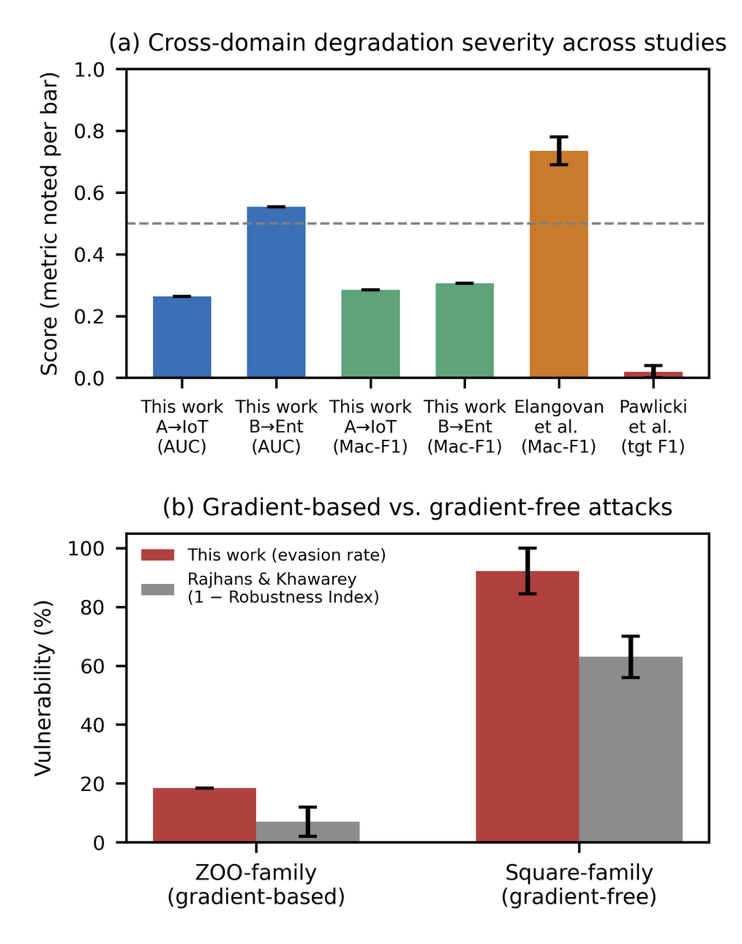
\includegraphics[width=0.48\textwidth]{fig4.png}}

\caption{(a) Cross-domain degradation severity across studies; error bars for Elangovan et al.~[5] and Pawlicki et al.~[36] show the midpoint and half-width of each paper's own reported range, not a confidence interval. (b) Gradient-based vs.~gradient-free attack vulnerability, this work vs.~[14]; Rajhans \& Khawarey [14] bars are likewise the midpoint/half-width of their reported Robustness Index range, not a confidence interval.}

\label{fig4}

\end{figure}

The cgroup-proxy mean (4.31 ms) is numerically lower than that of Diab et al.'s [34] real-Raspberry-Pi-3B+ figure (22 ms) and Wijethilaka et al.'s [35] real-Raspberry-Pi-4 figure ($\sim$50 ms), and higher than Haruna et al.'s [38] Docker-based figure (0.41 ms, no percentiles reported); the comparison is an order-of-magnitude anchor rather than a controlled benchmark, since none of the four studies share the dataset, hardware, or pipeline composition used here.

\section{Conclusion and Future Work}

Using a single model that is jointly-trained on a shared canonical schema is not just an operational convenience over two domain-specific models --- it is actually stronger than a specific, mechanistically-understood failure mode (sign-inverted feature-outcome relationships across domains) that can cause naive domain-specific transfer to invert instead of being less accurate. The model's adversarial evasion surface is substantially larger than a preliminary assessment first indicated, but a SHAP-attribution drift monitor built from explanations already computed for interpretability flags the resulting evaded traffic as a batch-level distributional shift by a wide margin, at a bounded and measured edge-deployment cost.

This work has several limitations that bound its claims and motivate future work. Since enterprise-side adversarial robustness has not been tested, it is not reasonable to assume that the evasion rates above apply to the enterprise domain. Only three black-box attack families were tested, all on IoT-domain traffic. The reported evasion rate is a lower bound rather than a proven ceiling because neither an exact MILP-based attack nor a SHAP-guided attack against the drift monitor here have been tested. Future work should prioritize: validating the edge benchmark on physical Raspberry Pi hardware; identifying what drives the residual cross-domain gap that remains even after removing the two flagged mismatched features (Section V-B); extending adversarial evaluation to the Enterprise domain and testing SHAP-guided and physically-realizable (inter-feature-consistent) adversarial attacks against both the classifier and the drift monitor; re-calibrating the drift-monitor threshold against a larger pool of null batches and extending its evaluation to a larger number of shift batches; running a hyperparameter search for Models A/B/C to establish a fully-tuned performance ceiling; and measuring the operational cost of a two-model deployment against the single pooled model proposed here, to make the deployment argument in Section V-F concrete rather than narrative.

\begin{thebibliography}{00}
\bibitem{ref1} I. Sharafaldin, A. H. Lashkari, and A. A. Ghorbani, "Toward generating a new intrusion detection dataset and intrusion traffic characterization," in Proc. Int. Conf. Inf. Syst. Secur. Privacy (ICISSP), 2018, pp. 108--116.
\bibitem{ref2} E. C. P. Neto, S. Dadkhah, R. Ferreira, A. Zohourian, R. Lu, and A. A. Ghorbani, "CICIoT2023: A real-time dataset and benchmark for large-scale attacks in IoT environment," Sensors, vol. 23, no. 13, Art. no. 5941, Jun. 2023.
\bibitem{ref3} S. Layeghy and M. Portmann, "Explainable cross-domain evaluation of ML-based network intrusion detection systems," Comput. Electr. Eng., vol. 108, Art. no. 108692, May 2023.
\bibitem{ref4} S. Layeghy, M. Baktashmotlagh, and M. Portmann, "DI-NIDS: Domain invariant network intrusion detection system," Knowl.-Based Syst., vol. 273, Art. no. 110626, Aug. 2023.
\bibitem{ref5} R. Elangovan, D. D. Parthasarathy, M. Jawahar, P. Kaliyaperumal, B. Balusamy, S. Yogarayan, and V. Venkatesan, "Cross-dataset temporal and semantic generalization of intrusion detection models for the future internet," Future Internet, vol. 18, no. 4, Art. no. 194, Apr. 2026.
\bibitem{ref6} M. Cantone, C. Marrocco, and A. Bria, "Machine learning in network intrusion detection: A cross-dataset generalization study," IEEE Access, vol. 12, pp. 144489--144508, 2024.
\bibitem{ref7} J. Vitorino, I. Praça, and E. Maia, ``SoK: Realistic adversarial attacks and defenses for intelligent network intrusion detection,'' Computers \& Security, vol. 134, Art. no. 103433, 2023.
\bibitem{ref8} B. Nugraha, A. V. Jnanashree, and T. Bauschert, "A versatile XAI-based framework for efficient and explainable intrusion detection systems," Ann. Telecommun., vol. 80, pp. 1095--1120, Sep. 2025.
\bibitem{ref9} A. Tziouvaras, B. Bertalanič, G. Floros, K. Kolomvatsos, P. Sarigiannidis, and C. Fortuna, "A representation learning approach to feature drift detection in wireless networks," IEEE Trans. Emerg. Top. Comput., 2025.
\bibitem{ref10} D. Slack, S. Hilgard, E. Jia, S. Singh, and H. Lakkaraju, "Fooling LIME and SHAP: Adversarial attacks on post hoc explanation methods," in Proc. AAAI/ACM Conf. AI, Ethics, Soc. (AIES), Feb. 2020, pp. 180--186.
\bibitem{ref11} M. Wang, K. Zheng, Y. Yang, and X. Wang, "An explainable machine learning framework for intrusion detection systems," IEEE Access, vol. 8, pp. 73127--73141, 2020.
\bibitem{ref12} S. Barrett, G. Dorai, L. Li, and S. Rajaganapathy, "FADES: Adaptive drift estimation via conformal signals for streaming intrusion detection," Electronics, vol. 15, no. 10, Art. no. 2114, May 2026.
\bibitem{ref13} A. Kantchelian, J. D. Tygar, and A. Joseph, "Evasion and hardening of tree ensemble classifiers," in Proc. 33rd Int. Conf. Mach. Learn. (ICML), 2016, pp. 2387--2396.
\bibitem{ref14} M. Rajhans and V. Khawarey, "Beyond gradient-based attacks: Adversarial robustness and explainability stability in cybersecurity classifiers," arXiv preprint arXiv:2607.01679, Jul. 2026.
\bibitem{ref15} M. Andriushchenko, F. Croce, N. Flammarion, and M. Hein, "Square attack: A query-efficient black-box adversarial attack via random search," in Proc. Eur. Conf. Comput. Vis. (ECCV), Aug. 2020, pp. 484--501.
\bibitem{ref16} J. Chen, M. I. Jordan, and M. J. Wainwright, "HopSkipJumpAttack: A query-efficient decision-based attack," in Proc. IEEE Symp. Secur. Privacy (SP), May 2020, pp. 1277--1294.
\bibitem{ref17} B. Sun, J. Feng, and K. Saenko, ``Return of frustratingly easy domain adaptation,'' in Proceedings of the Thirtieth AAAI Conference on Artificial Intelligence, vol. 30, no. 1, 2016, pp. 2058--2065.
\bibitem{ref18} B. Sun and K. Saenko, ``Deep CORAL: Correlation alignment for deep domain adaptation,'' in Computer Vision -- ECCV 2016 Workshops, vol. 9915, 2016, pp. 443--450.
\bibitem{ref19} Y. Ganin, E. Ustinova, H. Ajakan, P. Germain, H. Larochelle, F. Laviolette, M. Marchand, and V. Lempitsky, ``Domain-adversarial training of neural networks,'' Journal of Machine Learning Research, vol. 17, no. 59, pp. 1--35, 2016.
\bibitem{ref20} M. Mahbub, M. T. Riasat, T. Hamid, S. C. Sutradhar, and M. S. A. Khan, ``A minimalistic yet effective domain adaptation strategy for IoMT network intrusion detection,'' Discover Internet of Things, vol. 6, no. 1, Art. no. 28, 2026.
\bibitem{ref21} J. Wu, H. Dai, K. B. Kent, J. Yen, C.-Z. Xu, and Y. Wang, ``Open set dandelion network for IoT intrusion detection,'' ACM Transactions on Internet Technology, vol. 24, no. 1, Art. no. 4, 2024.
\bibitem{ref22} S. A. Almahaqeri, M. H. Almourish, A. A. Nasser, A. S. A. Alghawli, A. A. K. Elsayed, and A. N. Alhejoj, ``An optimized gradient boosting framework for IoT intrusion detection: A comprehensive evaluation on the CICIoT2023 dataset,'' Scientific Reports, vol. 16, no. 1, Art. no. 16909, 2026.
\bibitem{ref23} U. Ahmed, Z. Jiangbin, A. Almogren, M. Sadiq, A. U. Rehman, M. T. Sadiq, and J. Choi, ``Hybrid bagging and boosting with SHAP based feature selection for enhanced predictive modeling in intrusion detection systems,'' Scientific Reports, vol. 14, no. 1, Art. no. 30532, 2024.
\bibitem{ref24} G. Engelen, V. Rimmer, and W. Joosen, ``Troubleshooting an intrusion detection dataset: The CICIDS2017 case study,'' in 2021 IEEE Security and Privacy Workshops (SPW), 2021, pp. 7--12.
\bibitem{ref25} M. Sarhan, S. Layeghy, and M. Portmann, ``Towards a standard feature set for network intrusion detection system datasets,'' Mobile Networks and Applications, vol. 27, no. 1, pp. 357--370, 2022.
\bibitem{ref26} A. Tolay, ``Beyond detection accuracy: Measuring explanation cost, stability, and utility for resource-aware IoT intrusion detection,'' arXiv preprint arXiv:2608.10349, 2026.
\bibitem{ref27} T. Chen and C. Guestrin, ``XGBoost: A scalable tree boosting system,'' in Proceedings of the 22nd ACM SIGKDD International Conference on Knowledge Discovery and Data Mining, 2016, pp. 785--794.
\bibitem{ref28} B. Schölkopf, J. C. Platt, J. Shawe-Taylor, A. J. Smola, and R. C. Williamson, ``Estimating the support of a high-dimensional distribution,'' Neural Computation, vol. 13, no. 7, pp. 1443--1471, 2001.
\bibitem{ref29} S. M. Lundberg and S.-I. Lee, ``A unified approach to interpreting model predictions,'' in Advances in Neural Information Processing Systems 30, 2017, pp. 4765--4774.
\bibitem{ref30} S. M. Lundberg, G. Erion, H. Chen, A. DeGrave, J. M. Prutkin, B. Nair, et al., ``From local explanations to global understanding with explainable AI for trees,'' Nature Machine Intelligence, vol. 2, no. 1, pp. 56--67, 2020.
\bibitem{ref31} M. T. Ribeiro, S. Singh, and C. Guestrin, ``Why should I trust you?: Explaining the predictions of any classifier,'' in Proceedings of the 22nd ACM SIGKDD International Conference on Knowledge Discovery and Data Mining, 2016, pp. 1135--1144.
\bibitem{ref32} M.-I. Nicolae, M. Sinn, M. N. Tran, B. Buesser, A. Rawat, M. Wistuba, V. Zantedeschi, N. Baracaldo, B. Chen, H. Ludwig, I. M. Molloy, and B. Edwards, ``Adversarial robustness toolbox v1.0.0,'' arXiv preprint arXiv:1807.01069, 2018.
\bibitem{ref33} P.-Y. Chen, H. Zhang, Y. Sharma, J. Yi, and C.-J. Hsieh, ``ZOO: Zeroth order optimization based black-box attacks to deep neural networks without training substitute models,'' in Proceedings of the 10th ACM Workshop on Artificial Intelligence and Security, 2017, pp. 15--26.
\bibitem{ref34} A. Diab, A. Chehade, E. Ragusa, P. Gastaldo, R. Zunino, A. Baghdadi, and M. Rizk, ``Intrusion detection on resource-constrained IoT devices with hardware-aware ML and DL,'' in 2025 IEEE International Conference on Emerging Trends in Engineering and Computing (ETECOM), 2025.
\bibitem{ref35} R. W. K. S. Wijethilaka, K. Yapa, and D. Siriwardena, ``A cost effective machine learning based network intrusion detection system using Raspberry Pi for real time analysis,'' PLOS ONE, vol. 20, no. 12, Art. no. e0331123, 2025.
\bibitem{ref36} M. Pawlicki, S. Szelest, R. Kozik, and M. Choraś, "SHAP insights into domain adaptation in netflow-based network intrusion detection powered by deep learning," in Proc. Int. Conf. Availability, Rel. Secur. (ARES), 2025, pp. 292--309.
\bibitem{ref37} R. Kazoom, Y. Ratzabi, E. Rothstein, and O. Hadar, "Boundary on the table: Efficient black-box decision-based attacks for structured data," arXiv preprint arXiv:2509.22850, Sep. 2025.
\bibitem{ref38} A. Haruna, S. I. Yusuf, and S. A. Muhammed, ``Benchmarking lightweight ML models for edge-IoT botnet detection under resource constraints,'' FUDMA Journal of Sciences, vol. 10, no. 8, pp. 13--18, 2026.
\end{thebibliography}

\end{document}
